\chapter{Conclusion}\label{sec:conclusion}
\clearpage
This dissertation aimed to adapt pattern recognition methods employed in other fields (e.g., computer vision and machine learning) to environmental health data. We modified existing methods to address limitations or specifications that did not adapt well to circumstances typically found in environmental mixtures.  We included specific modifications to remove the researcher from pattern number selection or specification, to retain the interpretability of a parts-based representation of data, and to explicitly account for uncertainty in identified patterns. We further demonstrated how the quantified uncertainty could be incorporated in a hierarchical health model to understand the relationships between identified patterns of endocrine disrupting chemical (EDC) exposure and child cognitive development. In this final chapter, we discuss our findings and their implications in three main sections: in Section~\ref{sec:summarize} we summarize our findings and contributions and discuss their position within environmental mixtures and pattern identification research; in Section~\ref{sec:future} we discuss future research directions; and in Section~\ref{sec:ph} we conclude with the public health relevance and significance of our work.

\section{Our findings \& current research}\label{sec:summarize}

\subsection{Dissertation findings}\label{sec:findings}
We introduced two pattern identification methods adapted from computer vision and geological physics to environmental epidemiological research \citep{candes2011robust, zhou2010stable, holtzman2018machine}. We tailored principal component pursuit (PCP) and Bayesian non-parametric non-negative matrix factorization (\bnmfc) to better suit environmental data.

For PCP (Chapter~\ref{sec:ch2}), we began with the additive decomposition of an exposure mixture into a low-rank matrix containing consistent patterns of exposure across pollutants and a sparse matrix isolating unique or extreme exposure events \citep{candes2011robust, zhou2010stable}. We then incorporated two existing extensions, (1) a non-convex rank penalty that performs well with data that may not have a strong underlying low-rank structure \citep{netrapalli2014non, chen2020bridging}, and (2) a recent formulation of the objective function that removes the need for parameter tuning (\hl{ref Zhang}). We further included (1) a non-negativity constraint to enhance interpretability of identified patterns, (2) a modified algorithm to allow for missing values that correspond to incomplete data, and (3) a separate penalty for chemicals measured below the limit of detection (PCP-LOD). Introduction of the sparse matrix is especially novel in environmental health, as unusual or extreme exposure events are usually discarded or ignored by standard methods.

For \bnmfc (Chapter~\ref{sec:ch3}), we assumed the data generating process of non-negative continuous priors on pattern loadings and individual scores and a non-parametric sparse prior on the pattern number \citep{holtzman2018machine}. We extended the method by explicitly modeling the variational distribution for identified chemical loadings and individual scores. With this distributional information, we accounted for uncertainty in identified patterns. This is a notable addition to environmental mixtures research, as, to our knowledge, no pattern recognition methods commonly employed in this field include confidence in estimation.

We further designed a two-stage Bayesian hierarchical model to incorporate the uncertainty of pattern identification in the estimation of health effects of environmental exposure patterns (Chapter~\ref{sec:ch4}). We identified two patterns of prenatal EDC exposure corresponding with diet and personal care product use (Figure~\ref{fig:load}). The diet pattern expressed exposure to phthalates and BPA, and the personal care product pattern represented exposure to phenols, including parabens, and diethyl phthalate. One standard deviation increase in the diet pattern was associated with a decrease of 3.5 IQ points (95\% credible interval: -6.7, -0.3), on average, in female children but not in males (Tables~\ref{tab:reg} and \ref{tab:supreg}).

\subsection{Distinct methods}\label{sec:difference}
Introducing two pattern recognition techniques for use in environmental health begs the question: what are the practical differences between these methods? How would a researcher decide between them? The goal of both methods is to identify patterns in environmental mixtures that could represent sources or actions leading to exposure.  However, similar to the selection of mixture methods more generally, determining which tool better suits an analysis depends on the specific research question and the data at hand. For example, we would choose PCP-LOD if we believed that the data included sparse events or if many chemicals measurements were below the LOD. Additionally, PCP-LOD must be paired with another method to produce individual scores and chemical loadings similar to those obtained from \bnmfc, so the appropriateness of the second approach would also affect the decision. For instance, PCP-LOD paired with a clustering algorithm (e.g., k-means or hierarchical clustering) would partition individuals based on their chemical measurements (or transposed, partition chemicals based on individuals' measurements) \citep{friedman2001elements}. This may answer certain research questions concerning identification of subgroups (while isolating sparse events); however, cluster membership is categorical and may not clarify research questions regarding exposure degree or magnitude. Or as another example, PCP-LOD paired with singular value decomposition (SVD), as we did in Chapter~\ref{sec:ch2}, or principal component analysis (PCA) would not make use of the non-negativity constraint on the low-rank matrix, so it may not be suitable for research questions that emphasize interpretability of patterns.

We would choose \bnmf if we planned to include the identified patterns in a health model or if we required the variational approximation to the posterior for another reason. Still, circumstances exist, separate from the research question, in which neither method would perform well. If a mixture is not large enough, most pattern identification methods will fail to yield meaningful results. It is impossible to designate an exact cutoff for mixtures that are `too small' to employ pattern recognition techniques, however, because it simultaneously depends on the correlation structure between chemicals. For example, a mixture of five chemicals may be too small for any method to provide useful results, but if two chemicals are highly correlated and the remaining three are highly correlated (with minimal cross-group correlations), the resulting two pattern solution could be interpretable. These are general guidelines and not hard rules, as numerous elements of a study may influence the choice of analytical method. This subsection discusses PCP-LOD and \bnmfc, specifically; for comparisons with other methods, the reader should refer to Chapter~\ref{sec:ch1} for an introduction to more traditional pattern identification tools, Chapter~\ref{sec:ch2} for methods comparison with PCP-LOD, and Chapter~\ref{sec:ch3} for comparison with \bnmf.

\subsection{Environmental mixtures \& pattern recognition}
\label{sec:mixtures}
Research on environmental mixtures is advancing rapidly and these methods were reviewed in Chapter~\ref{sec:ch1}. Briefly, environmental health scientists and epidemiologists, in collaboration with biostatisticians, have adapted and applied numerous analytical methods from other fields. Standard machine learning methods such as penalized regression (lasso, ridge regression, and elastic net), deletion/substitution/addition, clustering (hierarchical and k-means), and tree-based methods (regression trees, random forests, and gradient boosting) have been employed to answer various questions concerning environmental mixtures \citep{tanner2020environmental, oskar2020machine, choirat2019data, vuong2020chemical, lazarevic2019statistical, coker2018multi, hamra2018environmental, huang2018cumulative, stafoggia2017statistical}. Other methods such as Bayesian kernel machine regression (BKMR) \citep{bobb2014bayesian, bobb2018statistical}, weighted quantile sum (WQS) regression \citep{carrico15}, quantile g-computation \citep{keil2020quantile}, SuperLearner (an ensemble machine learning technique) coupled with g-computation \citep{oulhote2019joint}, Bayesian factor analysis \citep{ferrari2020bayesian, bhattacharya2011sparse}, and Bayesian multiple index models have been designed or modified specifically for environmental data \citep{mcgee2021bayesian}. Notably, the majority of methods development within environmental health to date focused on supervised techniques, i.e., models where the health outcome informs the solution. This reflects the collective goal of environmental epidemiology to determine how environmental exposures impact human health.

Our work here concerns unsupervised methods where no health outcome influences the formation of identified patterns. As we have shown, our methods (and unsupervised methods, more generally) can be used in conjunction with human health models.  Furthermore, unsupervised methods are especially advantageous as a contribution to policy-relevant research because observed patterns may correspond with entities that are more receptive to regulation than individual chemicals and may be associated with multiple measures of health and disease. Pattern recognition in this context, however, introduces unique challenges and is in many ways a more difficult problem than regression or classification.

In supervised learning, we know the truth---the health outcome, in our case---or, at least, an approximation of it (if e.g., it is measured with error), and a clear measure of success, or lack thereof, exists. In the context of unsupervised learning, no such direct measure of success exists because we do not know the true patterns underlying an exposure mixture \citep{ISLR}. Put simply, it is harder to label something we do not know than to label something we do know. In experiments in Chapters~\ref{sec:ch2} and \ref{sec:ch3}, we simulated data that allowed us to ascertain the validity of inference drawn from PCP-LOD and \bnmf because we knew the truth (i.e., the simulated loading and score matrices that we generated). In applied work, the true patterns remain unknowable and researchers resort to heuristic arguments for judgments concerning the quality of results (e.g., researchers often try several parameterizations and choose the one with the most useful solution for their application) \citep{friedman2001elements}. We considered interpretability of the solution during the design of both models; still, a natural notion of a `good pattern,' or one that reflects reality, remains ambiguous. 

non-negative matrix factorization (NMF), the foundation for \bnmfc, introduces further complications. We found non-negativity desirable because of the enhanced interpretability of a parts-based representation and potentially correlated patterns \citep{lee1999learning, lee2001}. Chemical concentrations cannot be negative, and a negative amount of a chemical in a pattern or of a pattern in an individual does not correspond to presence or absence or intuitively convey exposure level. NMF, however, presents the additional obstacle of non-identifiability, where multiple decompositions are observationally equivalent \citep{donoho2004does}. Non-identifiability is a problem because multiple solutions are equally likely, but their interpretations are not necessarily similar. 

An NMF solution can only be unique up to scaling and permutation \citep{eggert2004sparse}. The solution multiplied by any matrix and its inverse (i.e., $W H = W M M^{-1} H$, where $M$ is an invertible matrix) remains equivalent \citep{xu2003document}. Or more simply, multiplying a pattern in the loading matrix by a constant and dividing the corresponding pattern in the score matrix by the same constant produces the same solution but can potentially vastly alter results. Our work does not change this inherent attribute of NMF, but we addressed it by normalizing all loadings matrices to have row-wise $\ell_1$ unit norms and scaling the patterns in the score matrices by the corresponding normalization constant. In this way, we express all scores and loadings on the same scale. While infinite solutions are numerically equal, this one allows for a standard interpretation and comparison between patterns. Moreover, algorithms are agnostic to the permutation of patterns, meaning patterns have no fixed ordering, and permuted solutions are equivalent \citep{celeux1998bayesian}. This may pose problematic in fully Bayesian implementations of Markov chain Monte Carlo (MCMC) to approximate the posterior distribution \citep{bda3}, but we circumvented this by implementing our model with a variational inference approximation \citep{blei2017variational}. Finally, non-separability of the data may cause non-uniqueness of the solution \citep{laurberg2008theorems}. However, separability is a fairly mild assumption about the pattern structure under which NMF may recover the truth \citep{arora2016computing}. In the context of environmental data, the exposure matrix is separable if there exists at least one chemical that loads solely on each pattern \citep{arora2012learning}. This usually holds in real-life environmental data, as in Sections~\ref{results_app}~and~\ref{sec.patterns}.

Further computational concerns exist on the algorithmic side, where an exact NMF decomposition is NP-hard, meaning there cannot exist an efficient algorithm to calculate it \citep{vavasis2010complexity}. Nonetheless, while an optimal reconstruction may be computationally intractable, algorithms exist to satisfactorily approximate it \citep{gillis2020nonnegative}. Despite analytical complications with NMF, in particular, and unsupervised learning, in general, we employed these methods to answer questions ill-suited for supervised learning concerning inherent underlying patterns in a population.

We likewise encountered multiple challenges modifying PCP for environmental mixtures. We began our work with traditional PCP (i.e., stable PCP) \citep{candes2011robust, zhou2010stable}. We first struggled with how to determine the optimal value for $\mu$; this inspired the work in \hl{ref Zhang} to derive a universal choice of regularization parameter that yields near optimal performance across a range of noise levels in \rootpcpc. We then found that the default parameter values ($\lambda = 1/\sqrt{n}$ from \citet{candes2011robust}, and $\mu = \sqrt{p/2}$ from \hl{ref Zhang}) worked well for applications in computer vision but not for our own. To address this, we implemented a cross-validation approach with a grid across $\lambda$ and $\mu$ values. We next noticed that in our solutions, the low-rank matrices were too low-rank, where correlations within $\hat{L}$ were all approximately 1 and only one or two singular values were non-zero. We also found that the sparse matrices were not necessarily sparse; this was consistent with the rank issue, as PCP minimizes a weighted combination of the nuclear norm of $L$, $\|\boldsymbol{L}\|_{*}$, and the $\ell^1$ norm of $S$. After extensive experimentation, we determined that the nuclear norm was too strict for environmental data; or rather, the nuclear norm expected a strong low-rank structure that was present in computer vision but not in environmental applications. To address this, we replaced the nuclear norm with a rank-$r$ projection \citep{netrapalli2014non, chen2020bridging}, which improved performance on the low-rank matrix (though the sparse matrix remains not-that-sparse). The rank-$r$ projection requires the desired rank as an argument, so we added rank to the cross-validation procedure; while non-convex \rootpcp (\ncpcpc) still has parameters $\lambda$ and $\mu$, one of them may be set as a constant without a loss of generality because the nuclear norm (previously with a fixed coefficient of 1) is no longer present. In practice, this means that the cross-validation need only include rank and $\mu$ with $\lambda$ fixed at $1/\sqrt{n}$, or equivalently, we defined $\gamma$ as $\lambda$/$\mu$ and tune $\gamma$ and rank through cross-validation. Finally, we realized that \ncpcp and PCP-LOD were not converging for a large subset of the parameter-rank grid. To address this, we improved the algorithm with a proximal gradient method and initialization at the best rank-$r$ approximation. This improved convergence; however, it does not currently include the separate LOD penalty, the non-negativity constraint, or the square root formulation of the objective function.

\section{Future research directions}\label{sec:future}
To date, environmental epidemiological investigations of multi-pollutant exposures have asked a variety of research questions and developed and adapted numerous statistical and machine learning methods to address them. However, a number of important questions remain unaddressed and new challenges have become apparent. Below, we outline several opportunities for future research on environmental mixtures and pattern identification therein.

\subsection{Future extensions}\label{diss:future}
This dissertation detailed work to adapt two pattern identification methods for use in environmental mixtures research. Both tools, however, should be considered works-in-progress. We plan to incorporate various methodological extensions and to apply these methods to future research questions concerning mixtures in independent study populations.

For PCP-LOD, we envision several elements that would improve performance in certain areas. First, as we emphasized in Chapter~\ref{sec:ch3}, when characterizing multi-pollutant exposures for use in health studies, it is important to quantify the uncertainty in their estimation and propagate it in the health models. We propose, therefore, to extend PCP-LOD by coupling it with a bootstrap process to quantify and propagate uncertainty associated with the estimation of the low-rank and sparse matrices \citep{mak14_unc}. Second, we aim to allow for clustering and repeated measures, e.g., children within schools or sequential measurements within a person, which will be correlated. As currently implemented, the Frobenius norm in the error term $\left( \|L+S-X\|_{F} \right)$ is not able to reflect this structure. Clustering information can be incorporated into a hypergraph, and error can be measured in a metric which reflects the smoothness of the noise with respect to the hypergraph---i.e., the Laplacian metric \citep{zhou2006learning, kaminski2019clustering}. At the same time, we aim to incorporate this clustering information into our estimation of S. For instance, since S captures rare events in the environment, it is possible that these events will occur in subjects living in close proximity. We will leverage ideas from hierarchical sparse modeling to this end, treating entries in S that belong to the same group as a group of variables, and penalizing both the sum of $\ell_2$ norms of the groups, as well as the $\ell_1$ norm within each group \citep{yan2017hierarchical, sprechmann2011c, jenatton2011proximal}.

For \bnmf we anticipate future work to reformulate the two-stage hierarchical health model as a fully supervised model where the outcome of interest informs the `grouping' of the chemicals in the mixture. As a Bayesian model, \bnmf can be naturally embedded in a more complex model to estimate pattern-specific health effects \citep{bda3}. Although such an approach would not necessarily be helpful in informing regulatory action, as different groupings could be formed depending on the health outcome, it may provide insight on the potential biological pathways, especially in exploratory analyses when biological plausibility has not yet been established. This structure should also serve to enhance reproducibility, as identified patterns based on biological mechanisms would be more similar across populations than those identified by the current iteration of \bnmfc.

The patterns found in Chapters~\ref{sec:ch2} and \ref{sec:ch3} correspond well with known sources, behaviors, toxicity and chemical structure. Nevertheless, we do not yet know whether identified patterns will generalize to other populations. Future studies in separate study populations will better determine the generalizability of observed patterns. The NHANES data used in Chapter~\ref{sec:ch2} represent the general non-institutionalized US population; however, we did not account for the complex sampling design and weights of the study \citep{johnson2013national}. Oversampling was performed for adolescents (aged 12–19), older Americans (aged 60 and over), Mexican-Americans, African-Americans, pregnant women, and individuals at or below 130\% of the poverty level \citep{curtin2012national}, and PCP-LOD-identified patterns may represent sources or behaviors distinct to included participants. Similarly, the Mothers and Newborns cohort studied in Chapters~\ref{sec:ch3} and \ref{sec:ch4} is composed of low-income Dominican and African American mothers living in an urban environment, and the \bnmfc-identified EDC patterns may represent sources or behaviors distinct to this group. To address the potential limitation of generalizability of our current findings, future studies should attempt to replicate results in independent study populations. Exactly replicating patterns across different populations it is highly unlikely; however, similarities and differences between groups both contribute to a better overall understanding of exposure.

\subsection{Cross-disciplinary collaboration}
PCP-LOD and \bnmf have many benefits over standard pattern identification methods in environmental health; however, they cannot answer all mixtures-related research questions. Notably, neither method provides evidence for biological pathways between exposure mixtures and disease. In the previous section (Section~\ref{diss:future}), we discussed a potential extension to include \bnmf in a supervised model where the health outcome informs the pattern recognition process. Cross-disciplinary collaboration with toxicological research could provide another means of identifying biological responses to observed patterns. We propose to complement our epidemiological findings by exposing animal models to human-relevant mixtures. A coupled relationship between epidemiology and toxicology allows for a unified investigation of adverse relationships between exposure and disease \citep{adami2011toxicology}.

A growing body of work in this area already exists. Rodents and zebrafish, for example, offer opportunities to classify relevant human exposures, to identify chemical targets, and to reveal mechanisms underlying toxic responses \citep{vaz2019zebrafish}. Recent research has exposed mouse models to a human exposure-based mixture designed to reflect dietary exposure of persistent organic pollutants (POPs) in relation to gene expression \citep{myhre2021maternal}, colorectal cancer \citep{johanson2020maternal}, and stress \citep{hudecova2018human, berntsen2017design}. Similar work has exposed rat models to multiple defined mixtures of high-end human-relevant EDCs in relation to reproductive development \citep{johansson2020calretinin, isling2014late, axelstad2018edc, johansson2016perinatal, ramhoj2018perfluorohexane, christiansen2012mixtures, axelstad2014mixtures}. As another example, researchers are investigating toxicity mechanisms of environmental chemicals in zebrafish \citep{vaz2019zebrafish}. Advances in high-throughput screening approaches allow researchers to assess thousands of individual chemicals and permit rapid assessment of chemical mixtures \citep{tanguay2018rise}. Recent studies have exposed zebrafish to environmentally-relevant mixtures constructed from prevalent toxicants \citep{geier2018systematic} as well as an environmental mixture passively sampled from a contaminated ecosystem \citep{bergmann2017using, allan2012bridging} to study their relationship with developmental neurotoxicity.

A third model organism, the nematode worm, or \textit{Caenorhabditis elegans} (\textit{C. elegans}), demonstrates potential for use in the assessment of human-relevant mixtures, though there are not many studies to date \citep{hunt2017c}. One notable example of chemical mixture assessment with \textit{C. elegans} was conducted after a chemical spill in West Virginia in 2014. The National Toxicology Program (NTP) used \textit{C. elegans} (among other models) to evaluate the toxicity of 12 different compounds and chemical mixtures from the spill and found they had no effect on \textit{C. elegans} growth, development, feeding, or reproduction \citep{ntp_worms}. In addition, recent studies have investigated the toxicity of pesticide mixtures in \textit{C. elegans} \citep{wang2021assessing,huang2021combined}; however, these authors constructed binary mixtures of chemicals with similar modes of action, which leaves numerous avenues for future work.
 
Research efforts may be underway in other animal settings, as well. Specific organisms are suitable for studying certain traits, phenomena, and diseases, and the appropriate model depends on the health outcome of interest \citep{katz2016model}. We draw inspiration from the studies described. In collaboration with toxicologists, we can expose model organisms to identified patterns defined by the presence or absence of chemicals as well as their relative concentration compared with other mixture members. We can then explore biological targets and systems such as gene expression, transcriptomics, or metabolomics. While neither method proposed in this dissertation incorporates information about biological mechanisms, combining this work with toxicological studies will allow us to explicitly test identified patterns to determine their toxicity. With this inter-disciplinary approach to characterize biological plausibility, we may better understand relationships between patterns of environmental chemical exposures and human health.

\subsection{Environmental mixtures of interest}
This work identified patterns underlying two environmental mixtures, one comprised of 21 PCBs, dioxins, and furans measured in the 2001--2002 cycle of NHANES and one of 17 phenols and phthalate metabolites measured in pregnant women in New York City between 1998 and 2006. These are two of an uncountable number of conceivable chemical mixtures. The vast expanse of environmental exposures and their potential combinations present opportunities for future research on pattern recognition within an array of environmental mixtures. 

Individuals in the U.S. are ubiquitously exposed to multiple classes of EDCs through common household consumer products \citep{gore2015edc}. EDCs, generally, are structurally similar to endogenous human hormones and may mimic or interfere with normal hormonal processes \citep{zoeller2012endocrine}. There has been increasing interest in EDCs over previous decades, and research has linked these chemicals with developmental, reproductive, neurological, and immunological problems \citep{solomon2000environment, meeker2012exposure, kabir2015review}. Notably, this research has largely investigated one EDC at a time, which does not represent real-life multi-EDC exposure. Because of the complexity of the endocrine system, which is comprised of multiple interrelated feedback loops \citep{diamanti2009endocrine}, the dose-response curves between EDC exposure and various health outcomes are not well-characterized, but there is some evidence of steeper slopes at lower concentrations \citep{vandenberg2012hormones}, i.e., low-level exposures may have more effect on certain health outcomes (though high exposures are recognized as more detrimental overall). Within environmental mixtures research, some analyses of EDC mixtures aimed to identify specific individual EDCs as toxic \citep{tanner2020early, loftus2021exposure}, which is a difficult undertaking because of the high correlations between many environmental EDCs and their structural similarities \citep{kavlock1996research}. We believe that investigating patterns of EDCs may alleviate some of the challenges of decoupling EDC exposure. Both mixtures investigated in this work were comprised of EDCs \citep{gore2015edc, van1998toxic}. In addition to PCBs, dioxins, furans, phthalates, and phenols, EDCs of interest include perchlorates \citep{nizinski2020perchlorate}, perfluoroalkyl and polyfluoroalkyl substances \citep{pfaswebsite}, phyto-estrogens \citep{yilmaz2020endocrine}, and polybrominated diphenyl ethers \citep{gibson2018effects}. The identification of underlying patterns of EDCs corresponding with actions or circumstances leading to exposure may inform interventions or regulatory action to curb exposure.

Another mixture of interest includes metals and metalloids, such as arsenic (As), cadmium (Cd), magnesium (Mn), mercury (Hg), and lead (Pb). A large body of literature exists linking environmental metal exposure with various health endpoints such as cardiovascular disease \citep{nigra2016environmental} and neurodevelopment \citep{henn2012associations}. In related work, we assessed the joint effects of co-exposure to As, Cd, Mn, and Pb on adolescent intellectual function and blood pressure, and explored potential beneficial effects of selenium (Se; an element known to lessen the overt toxicity of As \citep{levander1977metabolic}). We observed significantly negative associations between As and Cd (and null associations between Mn, Pb, and Se) and general intellectual ability (while accounting for other metals) as well as a significant decrease in Full Scale intelligence quotient with increased exposure to the entire metals mixture \citep{wasserman2018cross}. We further observed significantly positive associations between As and Mn (and null associations between Cd, Pb, and Se) and systolic blood pressure (SBP) and between As, Se, Pb, and Cd (and null associations between Mn) and diastolic blood pressure (DBP) as well as a significant increase in DBP with increased exposure to the metals mixture \citep{chen2019early}. Our previous work, however, did not investigate potential patterns of biomarkers of metals exposure in relation to adolescent intelligence or blood pressure.

Air pollution is an additional multi-pollutant exposure of interest. Research in source apportionment to derive information concerning ambient pollution sources and the amount they contribute to air pollution levels is more mature than the environmental mixtures field as a whole \citep{paatero94, sun2020positive, krall2017associations}. Nevertheless, there remain avenues for future work. For example, uncertainty propagation continues to prove challenging. While research exists to quantify the uncertainty associated with certain pattern recognition techniques in environmental health \citep{park2015part, gass2015ensemble}, the current norm is to include patterns or clusters as identified in health models \citep{austin2012framework, zanobetti2014health, sarnat2008fine, krall2017associations, basagana2016neurodevelopmental, siponen2015source, dai2016fine}. A previous study using source apportionment to assess air pollution source-specific impacts on cardiovascular admissions, \citet{mak14_unc} showed that failure to account for this uncertainty resulted in overestimated confidence in inference, potentially spurious findings, and disagreement across methods.

The previous paragraphs identify potential chemical mixtures of interest that are`'grouped' by different features (e.g., biological mechanism for EDCs, chemical class for metals, and exposure matrix for air pollution). Future studies should investigate patterns within similar multi-pollutant exposures, and we designed both PCP-LOD and \bnmf for scenarios such as these. Of course, mixtures research need not be limited to a single class of chemicals, or only to chemical stressors. It may incorporate markers of socio-economic status, demographic factors, nutrition, or built environment variables, to name a few. We can also conceptualize exposures from a more `exposomic' perspective which captures a diverse range of elements in addition to environmental chemicals, like dietary constituents, psychosocial stressors, lifestyle and physical factors (e.g., temperature, humidity, or noise), as well as their corresponding biological responses (e.g., in the form of RNA, metabolites, or proteins) \citep{vermeulen2020exposome}. Both PCP-LOD and \bnmf remain effective in exposomic-relevant scenarios which have many more exposure variables than observations. This is often the case in metabolomics, proteomics, and transcriptomics which may have thousands of features per individual. In fact, colleagues are currently using PCP (without the LOD extension) in exploratory analyses of metabolomic data with 12,000 unlabeled features. Furthermore, \bnmf stems directly from the NMF literature, and NMF methods are routinely applied to identify semantic features within corpora of documents with many more words than documents \citep{blei2003latent, paisley2014bayesian}. As currently implemented, however, neither of our methods accommodates binary or categorical data (e.g., socio-economic status or demographic factors); though the Bayesian hierarchical model built to incorporate \bnmf can include such factors as covariates. % Additionally, \bnmf is capable of decomposing a matrix of count variables (e.g., the number of exposure events per county over time), as the assumed data generating process is a Poisson distribution; though a combination of continuous and count variables in one exposure matrix has not been studied and may produce unexpected results.

\subsection{Reproducibility in science}\label{sec:repro}
There has been substantial discourse within the scientific community concerning the reproducibility of research \citep{baker20161}. A U.S. National Science Foundation (NSF) committee defined reproducibility as ``the ability of a researcher to duplicate the results of a prior study using the same materials as were used by the original investigator'' \citep{cacioppo2015social}. If a different researcher cannot run the same analysis with the same setup and get the same result, is the original work good science \citep{goodman2016does}? Reproducibility in epidemiology is made more complex by the ethical matter of personally identifiable information (PII); however, availability of the analytic code, as a minimum, allows other researchers to repeat the analysis on independently collected data \citep{peng2011reproducible}. Replication of results in a separate study population (i.e., corroboration of results using the same procedures on an independent dataset) strengthens evidence \citep{peng2006reproducible}.

Packaging code into reusable analysis software enables the dissemination of tools to facilitate future work more efficaciously. This is a good step toward establishing reproducibility \citep{collberg2015repeatability}. In the physical sciences, the correct and complete documentation of conditions, configuration, and details of laboratory operations is essential for validity; in the statistical sciences, the corollary is well-documented software, making packaging an important and necessary part of the scientific process. Subject to the ethical constraints of PII, researchers should endeavor to make computations reproducible for others \citep{barnes2010publish}. Analytic code and simulated data accompanying this work are publicly available on GitHub in three repositories: Chapter~\ref{sec:ch2} in \texttt{\href{https://github.com/lizzyagibson/Principal.Component.Pursuit}{Principal.Component.Pursuit}}, Chapter~\ref{sec:ch3} in \texttt{\href{https://github.com/lizzyagibson/BN2MF}{BN2MF}}, and Chapter~\ref{sec:ch4} in \texttt{\href{https://github.com/lizzyagibson/edc-patterns-wisc}{edc-patterns-wisc}}. We included the cleaned NHANES dataset with the code from Chapter~\ref{sec:ch2} because it is a publicly available dataset. We did not include the Mothers and Newborns cohort data accompanying analyses in Chapters~\ref{sec:ch3} and \ref{sec:ch4}. These data were collected with written informed consent of mothers (and assent of children at age seven) \citep{perera03}; this did not include consent to make their data publicly available. In fact, we have a `Certificate of Confidentiality' that prevents us from making these data available. Additionally, even limited `deidentified' datasets can become identifiable if enough variables are included \citep{narayanan2008robust}.

Further, we found in related work that details such as package version and software environment (e.g., R version) affect reproducibility of results in epidemiological studies \citep{nunez2020reflection}. Upgrading a platform or moving between computer environments should not obstruct replication or reproduction of results. Packaging and version control enable consistent inputs to produce consistent outputs \citep{wilson2014best}, which allows validation of analytic code by a third party. Both PCP-LOD and \bnmf include components to promote reproducibility further detailed in the following section (Section~\ref{diss:future}).

\begin{figure}[!ht]
\centering
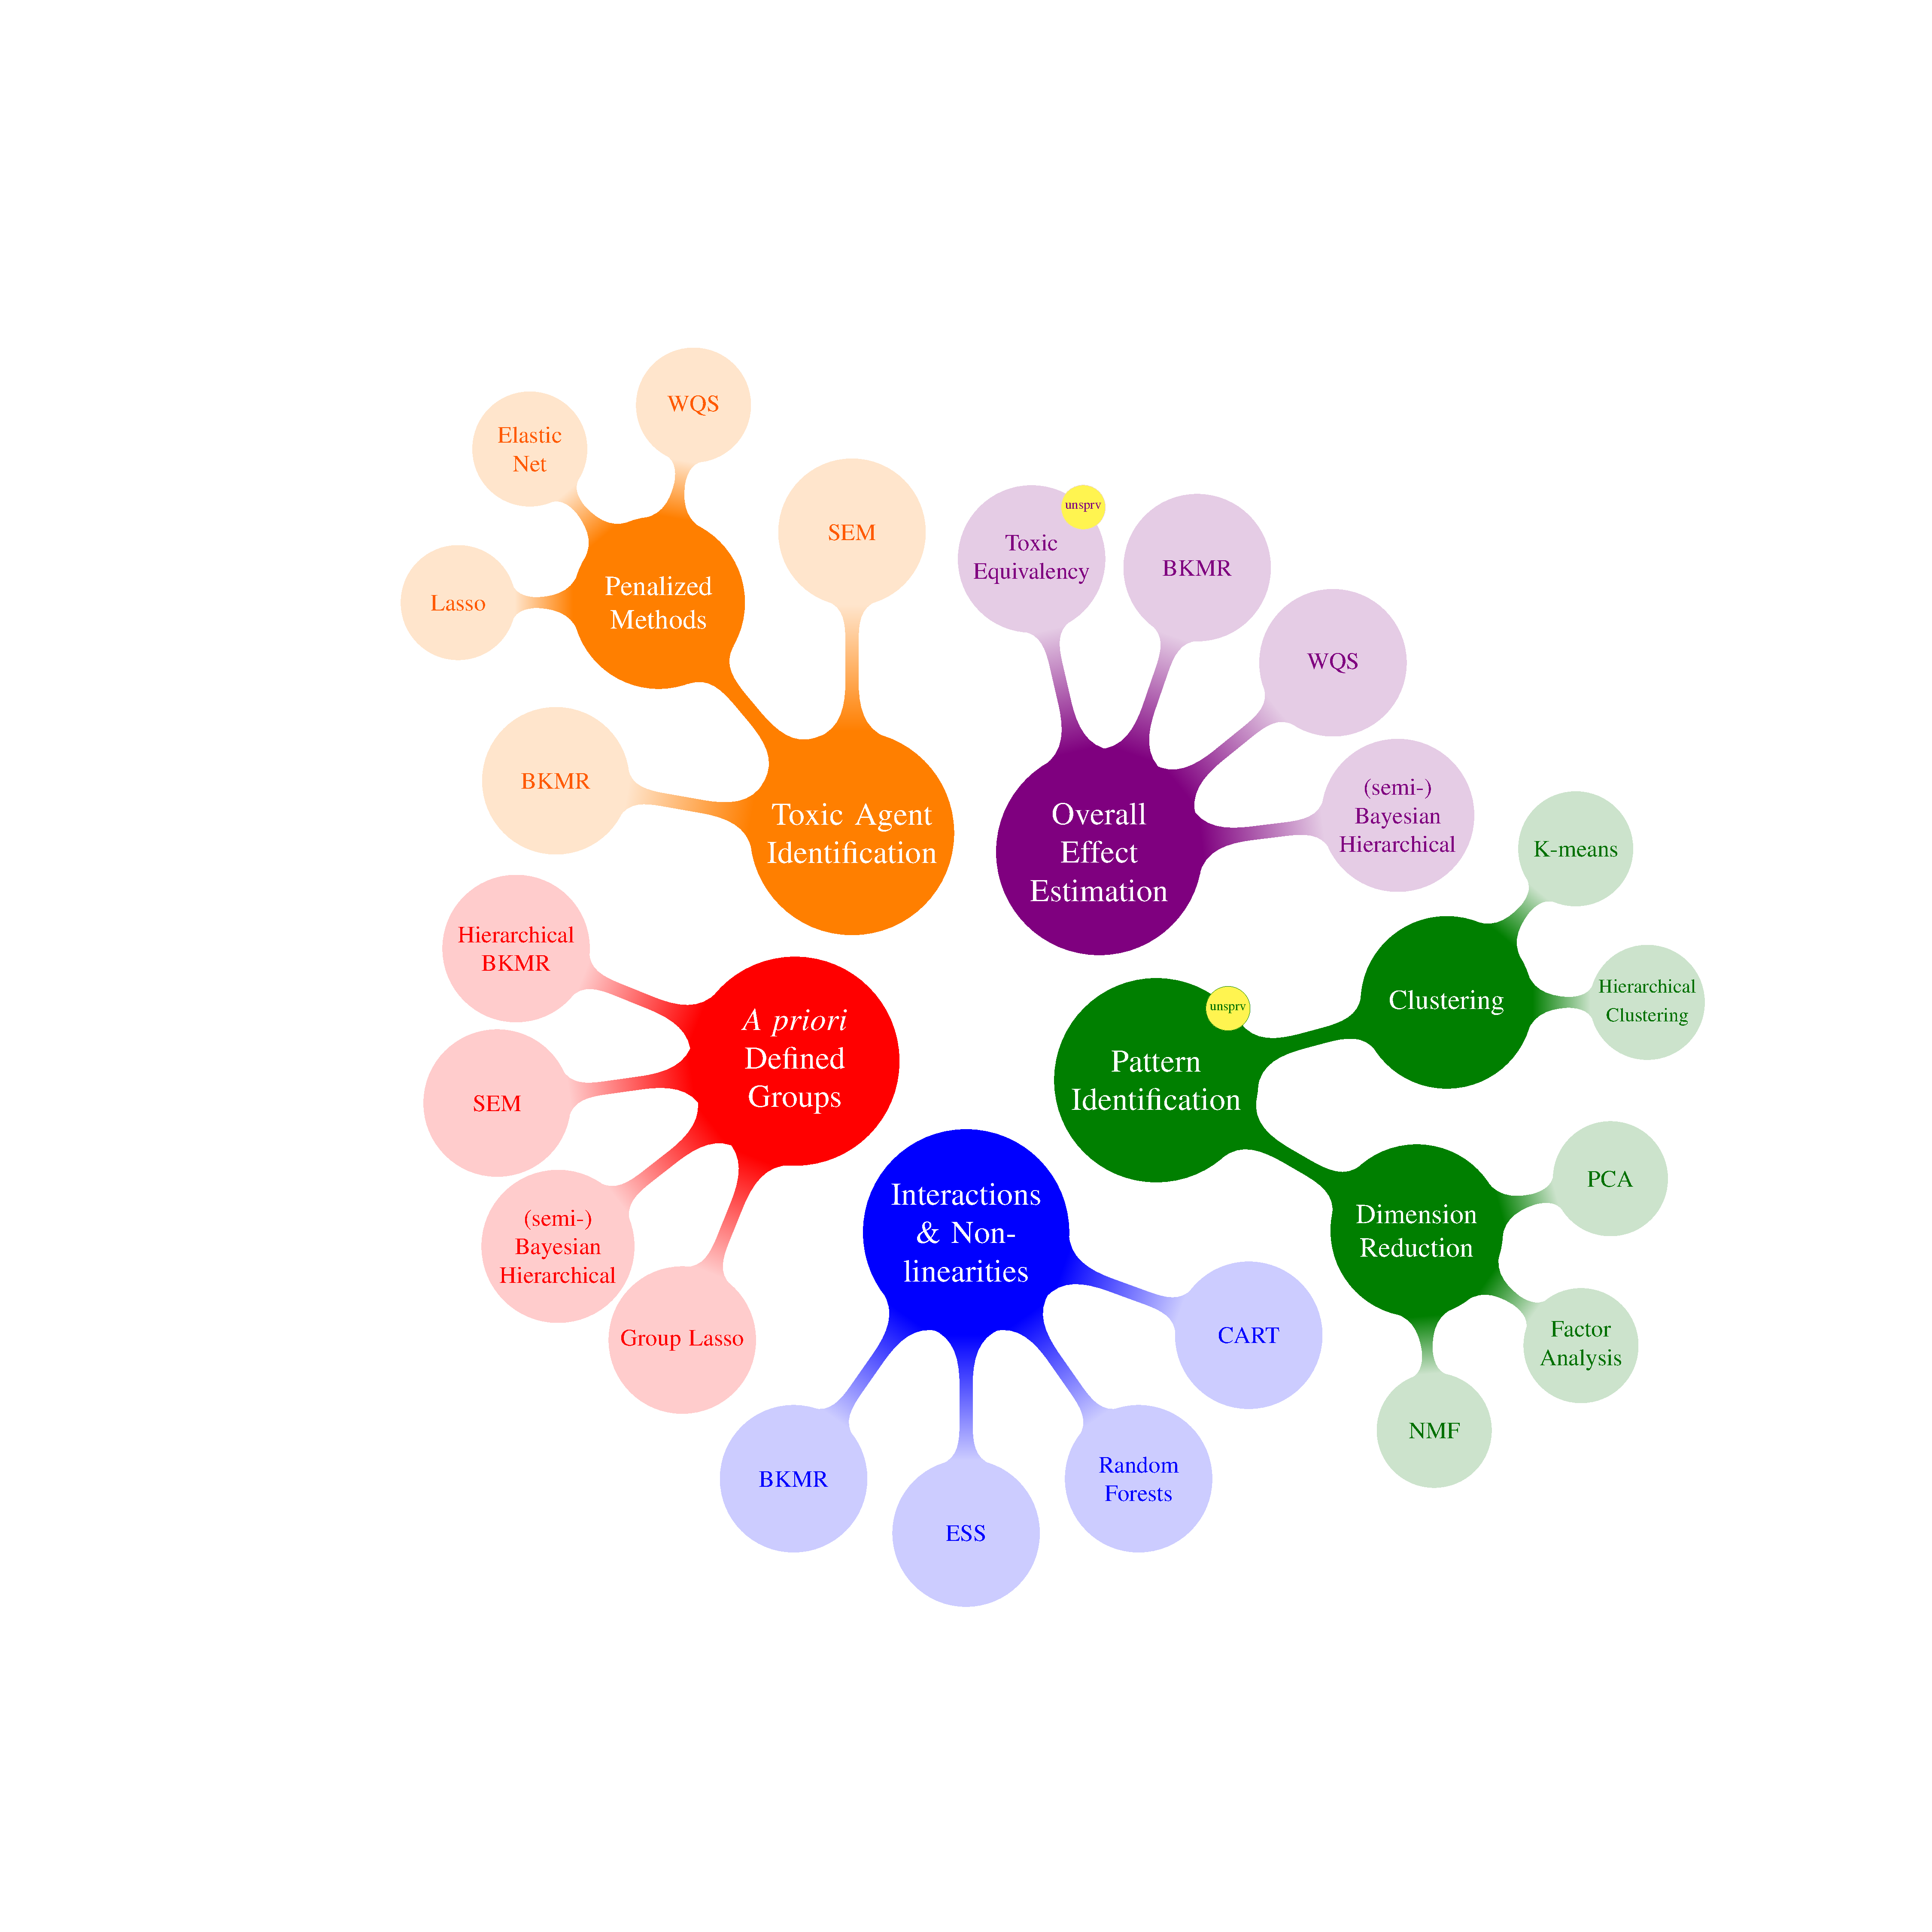
\includegraphics[scale = 0.286]{./figures/gibson_dissertation_image.pdf}
\caption{Potential classes of research questions concerning environmental mixtures. BKMR = Bayesian Kernel Machine Regression; CART = Classification and Regression Trees; ESS = Exposure Space Smoothing; Lasso = Least Absolute Shrinkage and Selection Opera; NMF = Non-negative Matrix Factorization; PCA = Principal Component Analysis; SEM = Structural Equation Modelling; WQS = Weighted Quantile Sum Regression.}
\label{fig:blobs}
\end{figure}

\subsubsection{Accessibility of methods}\label{diss:access}
Implementation of PCP-LOD and \bnmf employed sparse and low dimensional modelling, probabilistic machine learning, and complex optimization algorithms. Nevertheless, we developed both methods with the end user in mind. We took steps to remove the researcher from specification or selection of pattern number. We incorporated universal values for hyper-parameters in PCP-LOD so that users would not need to tune them. We chose vague priors for individual scores and chemical loadings in \bnmf so that they would suit various configurations of environmental data. We chose to approximate \bnmfc's posterior distribution through variational inference in part because it lifted the burden of assessing model convergence from the researcher. We mean for both methods to be broadly accessible to environmental health scientists and epidemiologists, who may lack formal statistical or mathematical training. Thus, as future work, we plan to develop and share user-friendly statistical software packages so that other researchers assessing exposures to mixtures can easily apply PCP-LOD or \bnmf to their research. Of course, users should understand what questions the methods were designed to address and their main assumptions, and we will include detailed documentation in the form of vignettes for guidance on proper use, inputs, interpretation, and limitations of both methods.

We propose to develop separate R packages for PCP-LOD (and other PCP implementations) and \bnmf to facilitate their use in environmental epidemiologic applications, along with developed synthetic datasets as examples. These will provide environmental epidemiologists with accessible and flexible tools to address study-specific needs. We believe that the existence of user-friendly packages, such as \texttt{bkmr}, \texttt{gWQS}, and \texttt{qgcomp}, encourages researchers to incorporate complex methodologies by making them more approachable \citep{bobb2018statistical, renzetti2016gwqs, keil2020quantile}. This work will also support our point in the previous section (Section~\ref{sec:repro}), as easily-accessible and well-documented packages will facilitate reproducibility of our results and of others'.

\section{Public Health relevance}\label{sec:ph}
\subsection{Research questions}\label{sec:question}
%\clearpage
A unifying theme in this work is the importance of the research question in driving the choice of statistical or machine learning method. For example, \bnmf cannot distinguish important individual mixture members or `bad actors,' and most regression-based approaches cannot identify underlying patterns of exposure. Further, the research question should be informed by the ultimate goal of the project---e.g., is it to provide evidence of a plausible biological pathway between chemical and disease or to support comprehensive regulation of chemicals that co-occur? In this dissertation, we introduced PCP-LOD and \bnmf as methods to better understand the underlying structure of environmental exposures.

Both are pattern recognition methods designed to address environmental health research questions concerning patterns of environmental exposures and to identify potential sources or behaviors leading to these exposures. The majority of environmental exposures are potentially modifiable, meaning that individual action or, more sustainably, regulatory action can prevent or (at least) reduce exposure. Accordingly, the fundamental aim of this work is to design methods capable of identifying actions or circumstances that contribute to simultaneous chemical exposures in support of targeted public health interventions and regulations. In Chapter~\ref{sec:ch4} we observed a negative association between a pattern of prenatal phthalate and BPA exposure and female child IQ at seven years of age. This finding supports public health and regulatory action on EDCs used as plasticizers and additives in food packaging; it does not support action against a single phthalate or a single phenol. Thus, this research supports a shift from chemical-by-chemical regulation toward \textit{class-based regulation}, where groups of chemicals identified as sharing properties and risks are evaluated and regulated together \citep{cordner2016can}.

\subsection{Public Health implications}\label{sec:fin}
No individual is exposed to a single chemical at a time. While public health research has traditionally relied upon standards such as linear and logistic regression to determine population-level associations between chemical exposures and outcomes, some research questions concerning multi-pollutant exposures require novel methods. The current focus on chemical mixtures represents a critical juncture in environmental health research. With this perspective, in Chapters~\ref{sec:ch2} and \ref{sec:ch3} we identified chemical patterns that we interpreted as sources of exposure within environmental mixtures; recognition of these patterns may aid in the development of preventive strategies to minimize exposure in individuals.

Researchers can use both PCP-LOD and \bnmf to provide foundational evidence for pattern-based regulatory action or informed interventions, where patterns may represent exposure source (e.g., diet as a source of POPs in Chapter~\ref{sec:ch2} and phthalates and BPA in Chapter~\ref{sec:ch3} and  \ref{sec:ch4}), at-risk behaviors (e.g., personal care product use contributing to phenol and DEP exposure in Chapters~\ref{sec:ch3} and \ref{sec:ch4}), or similar chemical structure (e.g., high or low molecular weight PCBs in Chapter~\ref{sec:ch2}). Both methods can be paired with expert knowledge to identify modifiable risk factors which are more effectively targeted than individual chemicals; for example, a source of particulate matter (PM), such as traffic, is more easily regulated than a single PM component.

Depending on the health outcome, implementation of strategies to reduce or prevent exposure to contributing environmental factors could have a consequential impact. In Chapter~\ref{sec:ch4} we considered the relationship between \textit{in utero} EDC exposure and child cognition. This work supports targeted public health interventions with expecting mothers or women contemplating pregnancy concerning their dietary choices. More importantly, confirmed associations between exposure patterns and neurodevelopment provide leverage to demand stricter governmental regulations of food packaging and actions to curb exposure.

Environmental health scientists and epidemiologists can use PCP-LOD and \bnmf to investigate shared sources of chemical exposure and behaviors and circumstances leading to exposure. We adapted these methods to suit environmental data (i.e., chemical concentrations) and to answer a subset of environmental mixtures questions. Research on underlying patterns of chemical exposure and unique or extreme exposure events can aid in the design and development of class-based regulations, informed policies, and targeted interventions to ensure equal access to a clean environment.
